
\chapter{Introduction}

\begin{quote}
{\it
  As soon as the Analytical Engine exists, it will necessarily guide the
  future of science. Whenever any result is then sought by its aid, the
  question will then arise -- by what course of calculation can these
  results be arrived at ... in the shortest time?}
\\\\
 -- Charles Babbage
\end{quote}

\section{Data Handling in Chemometrics}

\begin{doublespace}
In analogy to biometrics, econometrics and psychometrics, the practice of
chemometrics involves the extraction of chemically relevant information from
measurements taken from chemical systems \cite{wold:cils1995}.
Naturally, this process of information extraction relies on the construction of
mathematical models that describe a set of experimentally observed data, as
well as statistical frameworks that assign degrees of belief (probabilities)
to models, data, and their combinations:
\begin{equation*}
\mathbf{D} = f(\mathbf{D}) + \mathbf{E}
\end{equation*}

In this highly generalized equation describing chemometric modeling,
$\mathbf{D}$ is an experimentally measured dataset, $f(\mathbf{D})$ is
a mathematical model that recapitulates $\mathbf{D}$, and $\mathbf{E}$ is
the model `error', or variation in the measured data that is not
captured or described by the model. The ultimate goal of the analyst is to
generate a set of measured data $\mathbf{D}$ and construct a model
$f(\mathbf{D})$ that best describes that data (i.e. such that
$||f(\mathbf{D})|| \gg ||\mathbf{E}||$). The above general equation describes
a case of ``unsupervised'' chemometric modeling of the dataset $\mathbf{D}$,
but analysts may also choose to construct a supervised model, where the data
are used to predict a set of known responses $\mathbf{R}$:
\begin{equation*}
\mathbf{R} = g(\mathbf{D} \mid \mathbf{R}) + \mathbf{E}'
\end{equation*}
where the model $g(\mathbf{D} \mid \mathbf{R})$ extracts information from the
dataset that best describes $\mathbf{R}$, and the model error $\mathbf{E}'$
holds the differences between the known and modeled responses. Chemometrics
is intimately connected with the chemical systems it aims to describe, and
thus the exact choice of mathematical model and statistical framework depends
heavily on the particular problem, the data at hand, and the specific chemical
information desired by the analyst.
\\\\
As chemical systems under investigation increase in complexity, their
chemometric description requires a proportionally increasing amount of
measured data \cite{wold:cils1995}. Biochemical systems at the
levels of cellular metabolism and protein structure and function are
arguably some of the most complex systems available for study by
bioanalytical techniques, and demand vast amounts of spectral data
in order to be suitably described by chemometric models
\cite{
  wutrich:jmolb1982,
  kay:jmr2005,
  lindon:cmr2000,
  chen:rcms2006,
  han:metab2008,
  barding:jacs2012,
  baker:mmbio2012,
  marshall:metab2015}. Proper handling of these large datasets requires novel
tools and algorithms at each stage of the experimental process
(\figref{1.1}{Figure 1.1}) in order to ensure maximal information extraction
and minimal analyst errors.
\end{doublespace}

\begin{figure}[ht!]
\begin{center}
  \includegraphics[width=5in]{figs/intro/01-dataflow.png}
\end{center}
\caption
      [General Data Flow in Metabolomics.]{
  {\bf General Data Flow in Metabolomics.}
  \\
  Data in chemometric analyses of metabolism flows through this general graph,
  beginning at spectral data acquisition {\bf (0)}, through to loading and
  processing of instrumental data {\bf (1-3)}, further data treatment
  {\bf (4-5)}, mathematical modeling {\bf (6-7)} and model validation
  {\bf (8)}, and terminating on extraction of chemical information {\bf (9)}.
  In practice, this graph would be completely connected, and thus cyclic.
}
\label{figure.1.1}
\end{figure}

\subsection{Acquisition}

\begin{doublespace}
Nuclear Magnetic Resonance (NMR) spectroscopy is a popular analytical platform
for chemometric analyses of protein structure and cellular metabolism, due to
its ability to simultaneously report atomic-level details of the chemical
environments and motional dynamics of \hnmr{}, \cnmr{} and \nnmr{} nuclei in
biomolecules \cite{abragam1961,levitt2008}. While the amount of
information contained within one-dimensional (1D) NMR spectra is high, it is
commonly held in a relatively narrow spectral width
(e.g. -2.0 -- 16 ppm for \hnmr{} spectra). As a result, 1D \hnmr{} NMR spectra
of complex metabolite mixtures or biomacromolecules suffer from severe signal
overlap that confounds analysis and interpretation.
\\\\
Ever since the introduction of two-dimensional NMR methods by Jeener and Ernst
\cite{ernst:chim1975,maudsley:cpl1977} and the popularization of
three-dimensional methods for studying proteins by Bax and colleagues
\cite{marion:jacs1989,kay:bioc1989}, NMR spectroscopists have been
leveraging \hcnmr{} and \hnnmr{} connectivities to spread biomolecular
information from 1D \hnmr{} spectra into two or more dimensions. While
multidimensional experiments alleviate signal overlap, they require
significantly more time to acquire than 1D spectra, as any $D$-dimensional
experiment is effectively a $(D-1)$-dimensional array of $2^{D-1}$
one-dimensional experiments. Time constraints imposed by throughput
requirements, sample stability and instrumental maintenance have historically
forced spectroscopists to harshly undersample their multidimensional datasets
in the time domain, resulting in frequency domain digital resolutions much
lower than the intrinsic linewidth of their samples
\cite{szyperski:pnas2002,rovnyak:jbnmr2004}.
\end{doublespace}

\begin{SCfigure}
\includegraphics[width=3.5in]{figs/intro/02-sched.png}
\caption
      [Example Nonuniform Sampling Schedules on a 2D Nyquist Grid.]{
  {\bf Example Nonuniform Sampling Schedules on a 2D Nyquist Grid.}
  \\
  Nonuniform sampling schedules produced by ({\bf A}) stochastic and
  ({\bf B}) deterministic subsampling of a two-dimensional Nyquist sampling
  grid. Comparisons of the performance of such schedules are made in
  Chapter 2.
}
\label{figure.1.2}
\end{SCfigure}

\begin{doublespace}
In order to move from this ``sampling-limited'' regime of data acquisition,
the indirect dimensions of multidimensional NMR experiments may be nonuniformly
sparsely sampled (\figref{1.2}{Figure 1.2}), reducing the time required for
data collection while simultaneously enabling increased digital
resolution \cite{rovnyak:jmr2004}. When combined with non-Fourier
reconstruction algorithms such as Maximum Entropy, $\ell_1$-norm Minimization,
and Multidimensional Decomposition \cite{mobli:pnmrs2014}, this technique
of nonuniform sampling (NUS) is capable of producing high-quality,
high-resolution multidimensional spectra in a fraction of the time
required by traditional uniform sampling. However, the choice of which data
points to subsample from a uniform Nyquist grid is nontrivial and has typically
been made by random sampling methods
\cite{hoch:jmr2008,maciejewski:jmr2009}.
\end{doublespace}

\subsection{Processing and Treatment}

\begin{doublespace}
More often than not, effective chemometric modeling of raw experimental data
requires the data to be slightly modified from its original form. As an
example, two commonly utilized soft bilinear modeling algorithms, principal
component analysis (PCA, \cite{jolliffe2002}) and partial least squares
(PLS, \cite{wold1993}), analyze the eigenstructure of one or more data
matrices, and require subtraction of the sample mean and scaling by the sample
standard deviation in order to operate most effectively. When this modification
is instrumentation-specific, it is referred to as {\it processing}; otherwise,
it is considered a form of statistical {\it treatment}. The choice of which
processing and treatment methods to apply to a given dataset $\mathbf{D}$
varies, depending on how the data was collected, which model $f(\mathbf{D})$
is used, and what information is sought from the model by the analyst.
\\\\
Processing of NMR spectral datasets presents unique challenges to the analyst,
as each spectrum is collected in hypercomplex quadrature
\cite{schuyler:jmr2013} without absolute phase information. As a result,
NMR spectra must be phase-corrected to maximize the real spectral component
(cf. \hyperlink{chapter.3}{Chapter 3}). When multiple spectra are processed as
part of a statistical ensemble, any differences in phase {\it between} spectra
become a contributing factor to undesirable within-group variation that
inflates model errors. Thus, methods of phase-correcting multiple spectral
observations are required when those observations will become inputs into
multivariate modeling algorithms \cite{worley:cils2014}.
\\\\
Once instrument-specific processing has been performed on a dataset
$\mathbf{D}$, general statistical treatment operations may then be necessary,
depending on the model function $f(\mathbf{D})$ being utilized. One commonly
practiced method of preconditioning the eigenstructure of $\mathbf{D}$ for
PCA and PLS, known as binning or bucketing, involves partitioning $\mathbf{D}$
into smaller signal-containing spectral regions and integrating or vectorizing
those regions in order to achieve reduced data dimensionality. Multiple methods
of binning one-dimensional datasets have been developed, ranging from
na\"{\i}ve uniform subdivision algorithms
\cite{hedenstrom:cils2008,sousa:cils2013} to high-performance recursive
methods \cite{davis:cils2007,demeyer:anchem2008}. However, at the time
of this writing, no methods of intelligently (non-uniformly) binning
multidimensional datasets have been developed, essentially restricting bilinear
PCA and PLS modeling to using 1D \hnmr{} NMR spectral data in NMR chemometric
studies of metabolism.
\end{doublespace}

\begin{figure}[ht!]
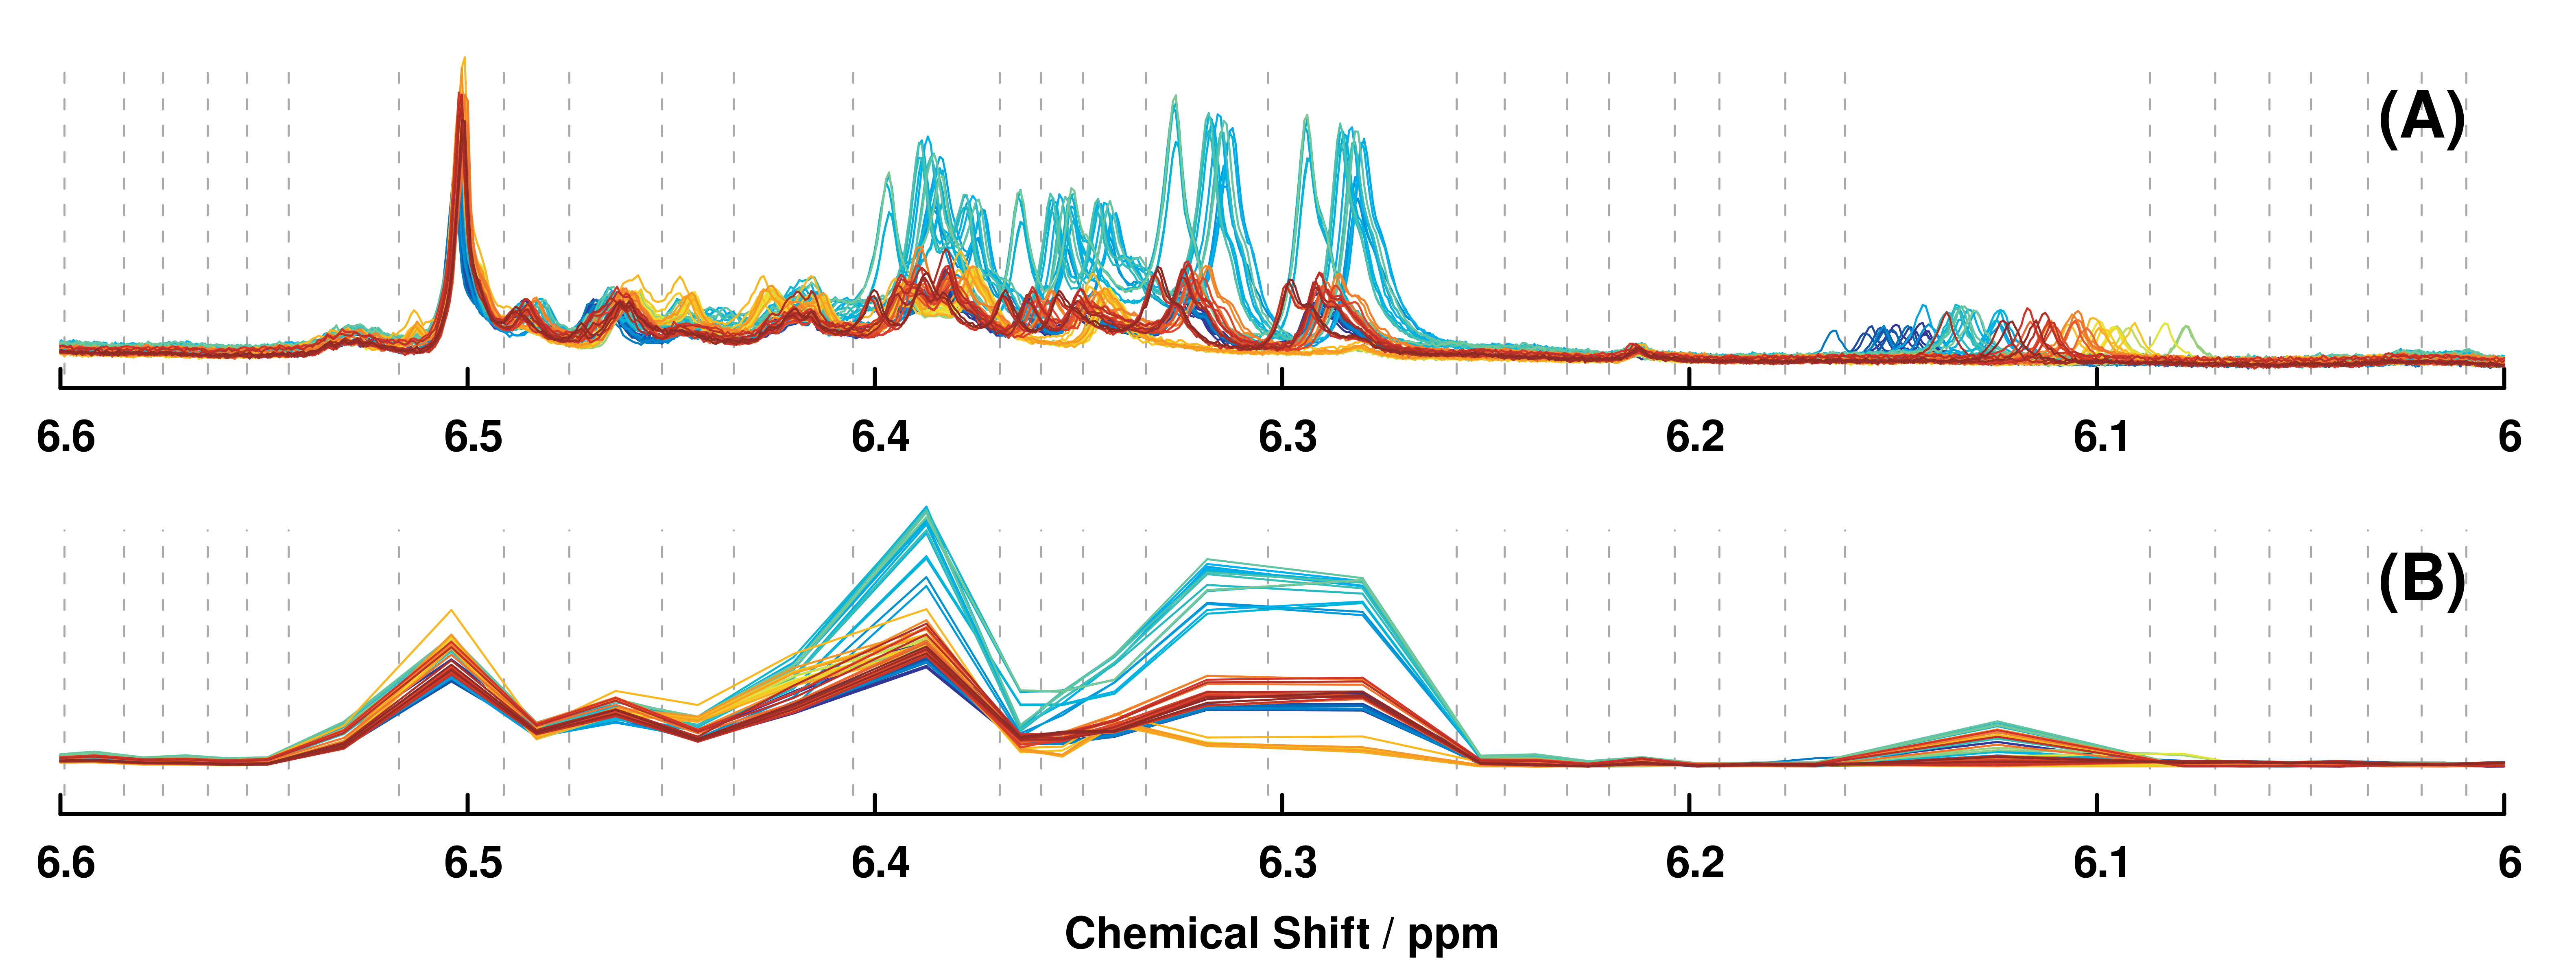
\includegraphics[width=6.5in]{figs/intro/03-bins.png}
\caption
      [Example Binning Result from a 1D \hnmr{} NMR Dataset.]{
  {\bf Example Binning Result from a 1D \hnmr{} NMR Dataset.}
  \\
  Full-resolution ({\bf A}) and adaptively intelligently binned ({\bf B}) 1D
  \hnmr{} NMR spectra from a chemometric study of brewed coffee roasts.
  Spectral color indicates the observation index, and dashed lines indicate bin
  boundaries. Further discussion of binning may be found in Chapters 3 and 6.
}
\label{figure.1.3}
\end{figure}

\subsection{Modeling and Validation}

\begin{doublespace}
Once a dataset $\mathbf{D}$ has been suitably processed and treated, a model
$f(\mathbf{D})$ may be trained on its contents. Within chemometrics, principal
component analysis (PCA) is undoubtedly the most routinely used modeling
algorithm for describing relationships between multivariate spectral
observations \cite{bro:anmeth2014}, because it provides an unbiased,
simplified picture of the data in a low-dimensional ``scores'' space. The
scores obtained from PCA models of spectral data are useful for determining
statistical distances between experimental groups
\cite{demaesschalck:cils2000,worley:abio2013}, which are effective predictors
of the reliability of any regression models that may be trained on the same
data.
\\\\
Another multivariate algorithm of equal popularity to PCA in chemometrics is
partial least squares (PLS), which is used for solving regression and class
discrimination problems on multivariate data \cite{wold1993}. While PLS
provides a similar low-dimensional scores-space view of spectral observations,
its true power in chemometrics lies in its ability to report ``loadings'',
which are spectral contributions that predict a set of chemical properties.
\\\\
The combination of PCA and PLS as a methodology for studying complex spectral
datasets has proven highly useful in chemometrics, most notably so in the
field of metabolomics \cite{lindon:cmr2000}. However, analysts must take care
when using models produced by these methods, as they have not been determined
using standard (over-determined) least-squares methods and may over-fit a
dataset at the expense of generality, which is required for broad inference
\cite{westerhuis:metab2008a}. Rigorous application of cross-validation methods,
including internal and external cross-validation
\cite{xu:cils2001,eshghi:cils2014}, response permutation testing
\cite{golland:learn2005} and CV-ANOVA \cite{eriksson:jchemo2008}, is required
in order to ensure that trained multivariate models are reliable and
generalizable to later measurements.
\end{doublespace}

\subsection{Inference}

\begin{doublespace}
Once multivariate models have been trained and validated on a given dataset,
they may finally be utilized for the extraction of chemical information from
that dataset. Often, this process of inference revolves around the analysis of
separations between one or more experimental groups in PCA or PLS scores space.
Because scores-space separations are often used as justification for further
costly experimentation, it is important to quantitatively measure these
separations using proper statistical tools \cite{worley:abio2013}.
\end{doublespace}

\section{Summary of Work}

\begin{doublespace}
By and large, this dissertation follows the logical flow of a data analyst
in the field of NMR metabolomics, working from methods in compressive data
acquisition, through a description of multivariate analysis techniques, to
processing, treatment and validation of multivariate modeling results, and
ending with a solution to a bioinformatics data handling problem: the
correlation between high-resolution protein structure and backbone chemical
shifts.
\\\\
\hyperlink{chapter.2}{Chapter 2} begins by introducing a gap-based nonuniform
sampling framework that provides several attractive advantages over traditional
probability density-based nonuniform sampling methods. While most methods of
generating nonuniform sampling schedules rely on randomly sampling from a
specified weighting function that is defined over a Nyquist grid, this new
method of gap sampling builds up schedules based on the value of a `gap
equation' that specifies the spacing between sampled Nyquist grid points. The
gap sampling framework is first defined, and comparisons in performance are
made between specific forms of gap sampling and the stochastic Poisson-gap
sampling method from Hyberts and Wagner \cite{hyberts:jacs2010}.
\\\\
A comprehensive description of the required data handling tasks -- steps
{\bf (1-9)} in \figref{1.1}{Figure 1.1} -- in metabolic fingerprinting and
untargeted metabolic profiling studies is provided within
\hyperlink{chapter.3}{Chapter 3}. Additional practical guidelines on the
relationship between class separations in PCA scores space and reliability
of OPLS-DA models on the same data are also presented. Examples of applied
multivariate analysis in metabolomics are given in
\hyperlink{chapter.4}{Chapter 4}.
\\\\
\hyperlink{chapter.5}{Chapter 5} introduces the MVAPACK toolbox for
chemometrics as a complete solution to the data handling problem in NMR-
and MS-based metabolomics studies. Beginning with a set of raw free induction
decays from an NMR spectrometer, analysts may now rapidly and easily generate
validated multivariate models using rigorously tested and peer-reviewed
routines in MVAPACK. As a result, both the turnaround time between data
collection and interpretation and the likelihood of analyst error are
dramatically reduced when using MVAPACK. The architecture and design rationale
of the MVAPACK toolbox are discussed in this chapter.
\\\\
\hyperlink{chapter.6}{Chapter 6} and \hyperlink{chapter.7}{Chapter 7} focus on
a novel method of data processing (Phase-scatter Correction) and describe its
application on datasets acquired from both metabolomics and high-throughput
protein-ligand affinity screens. \hyperlink{chapter.8}{Chapter 8} introduces
a novel method of data treatment (Generalized Adaptive Intelligent Binning)
that enables the direct use of multidimensional data tensors in PCA and PLS
modeling. Both phase-scatter correction and GAI-binning were developed within
the MVAPACK toolbox, which was specifically for efficient management of NMR
spectral data.
\\\\
\hyperlink{chapter.9}{Chapter 9} introduces the multiblock orthogonal
projections to latent structures (MB-OPLS) modeling method for handling
predictive and non-predictive variation in a set of observed data matrices.
Moving from modeling to inference, \hyperlink{chapter.10}{Chapter 10} describes
a small set of portable utilities that generate statistically sound dendrograms
of scores-space class relationships using both bootstrap-based and parametric
methods.
\\\\
\hyperlink{chapter.11}{Chapter 11} outlines the generation of a set of
bioinformatic tools to analyze the relationship between the geometry of
interacting pairs of carbonyls in protein backbones and their \cnmr{} chemical
shift values \cite{worley:pone2012}. These tools, combined with quantum
chemical computations, provide strong evidence for the nonexistence of
\npistar{} interactions between these carbonyl groups in native protein
structures.
\\\\
Finally, \hyperlink{chapter.12}{Chapter 12} summarizes the solutions provided
herein to a set of chemometrics and bioinformatics data handling problems and
discusses challenges and avenues of effort that will be required to solve
future problems of the same kind.
\end{doublespace}

\bibliographystyle{abbrv}
\bibliography{bworley}

